\chapter{Architectural Overview}

Figure~\ref{fig:architecture}
depicts important components
in the system and their relationships. This is an \adhoc diagram. The
boxes represent programs or people doing something or that react when
signaled. The arrows represent signaling or data transfer.

\begin{figure}[hbt]
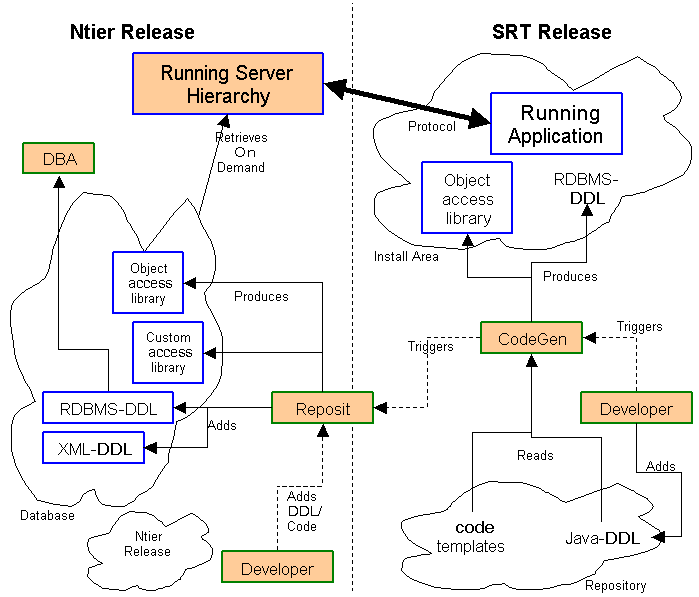
\includegraphics[width=\textwidth]{architecture.png}
\caption{Architecture of the \frontier system.\label{fig:architecture}}
\end{figure}

\section{Coupling}

Minimal logic in the client application.  Rules governing access to
objects/tables must be able to evolve independent of a client release.
Old clients must not prevent improvements or enhancements to newer
client applications.

\section{Protocol}

The protocol should allow prefetch algorithms in low-level servers to
add information that the server suspects you will be asking for in the
near future to current requests. If caching in middle layers of the
ntier system is down strictly on URL, this extra data may or may not
be present at some middle server. It may be a good idea to cause
cached URL expirations at a timely rate so that this newly added data
just appears like modified web pages.

It is possible to support general tabular data access in the
protocol. In other words, ntuple-like objects from database
tables. The result of such a query would include a description of the
data returned.

\subsection{Objects within a Server}

The server can be thought of as a collection of objects.  Each object has
a number of "get" methods that allow the user to ask for portions of data
within that object.  The arguments to the get methods are a set of keys.
The data returned is all the ``rows'' that match the set of keys.
Each object will have a type definition.  Users of this system must
supply type definitions or descriptions so that the server knows what
to deliver.  These definitions identify several important features:

\begin{enumerate}
\item the \emph{name} and \emph{version} of this type
\item the \emph{names} and \emph{types} of the attributes that will be
returned
\item the combinations of attributes that form \emph{keys}
\item an implied \emph{order} in which attributes are gaurenteed
to be delivered
\end{enumerate}

In addition to the things listed above, it may be worthwhile allowing
information that is domain specific, such as connecting this type
to a namespace or identifying SQL statements that can be used to
retrieve the information efficiently from a database.  Data type 
definitions will be in XML.

Below is the definition of the XML protocol which defines a single query
to a table or tables. 

\begin{verbatim}

<descriptor type="calibrunlist" version="1" xsdversion="1">
  <attribute position="1" type="int" field ="calib_run"/>
  <attribute position="3" type="float" field="calc_value"/>
  <attribute position="2" type="long" field="calib_version"/>
  <select>cr.calib_run, cr.calib_version, func(n)</select>
  <from>calibrunlist cr</from>
  <where>
    <clause>cid=@parm</clause>
    <param> position="1" type="int" key="cid"/>
  </where>
  <where>
    <clause>run=@param and xyz=@param</clause>
    <param position="1" type="int" key="run"/>
    <param position="2" type="string" key="xyz"/>
  </where>
  <final>order by ..... desc</final>
</descriptor>

\end{verbatim}

\begin{enumerate}
\item \emph{descriptor} - Top level tag describing what the data is for.
\begin{itemize}
\item \emph{type} - Name of the specific object this descriptor is for.
\item \emph{version} - Version number of the object.
\item \emph{xsdversion} - The version of XML servicer descriptor protocol which is being used 
to process the descriptor.
\end{itemize}
\item \emph{attribute} - Describles a datum which is being returned. The datum will be marshed 
according to the order of the \emph{attribute} tags.
\begin{itemize}
\item \emph{position} - The location of the datam in the \emph{select} tag this \emph{attribute}
is decribing.
\item \emph{type} - How the data will be marsheled out.  This is also the value returned when 
the client requests a description.  Valid values are:
\begin{itemize}
\item \emph{int}
\item \emph{long}
\item \emph{double}
\item \emph{float}
\item \emph{string}
\item \emph{bytes}
\item \emph{date}
\end{itemize}
\item \emph{field} - The name of the filed provided to the client when asked for a description.
\end{itemize}
\item \emph{select} - The fields returned from a query.
\item \emph{where} - A wrapper around tags which describe a specific where clause.  There may be 
multiples of this  tag.  The application decides on the \emph{where} to use based on the keys 
provided in the URL.
\item \emph{clause} - The SQL for the where clause, without the word ``where'', This will be used 
in the query.  Parameters may be passed in by useing the keyword ``@param''.  
\item \emph{param} - Identifies which ``@param'' keyword to replace with what value.
\begin{itemize}
\item \emph{position} - Which keyword to replace with this parameter
\item \emph{type} - How that keyword string is to be translated.  Valid values are
\begin{itemize}
\item \emph{int}
\item \emph{long}
\item \emph{double}
\item \emph{float}
\item \emph{string}
\item \emph{date}
\end{itemize}
\item \emph{key} - What key, supplied on the URL, which is being substituted into the parameter.
\end{itemize}
\item \emph{final} - Any final SQL clause which should be included in the query.

\end{enumerate}

In this definition a single description contains one select.  That select may have multiple where
clauses.  The where clause is chosen based on the keys provided in the URL.  Consideration was given
to allowing multiple selects in a description.  This has not been included due to the amount of 
effort required versus the amount of expected use.  

Consideration was also given for adding a second descriptor which defines how to convert the data
from the result set to the user object.  This has been put off to keep the initial implemention
fairly straight forward.  It may be added in the future.  The tag \emph{xsdversion} was added to 
make these changes possible.


\subsection{Nature of the returned data}

The structure of returned data is tabular and
record-oriented, very much like a table in a relational database or that
of a spreadsheet.
A significant difference is that the \emph{atoms} of the row can include
arrays of both fixed and variable size of fundamental \cpp
types\footnote{``Fundamental types'' include all primitive types and
also strings.}.  The type definition describes a single row, the
returned data is a collection or sequence of these rows.

We imagine supporting three types of data representations:
\begin{enumerate}
\item BLOB
\item CSV
\item XML
\end{enumerate}

Example data used for the next sections:
\begin{verbatim}
struct Thing { int i; string s; short h[3] };
vector<Thing> v(2);  // <----- we want to receive this

// values as we want to see them in memory at the end
Thing* t = { {1, "scum", { 0x5555, 0x6666 } },
             {2, "swine",{ 0x7777 } }
           };
\end{verbatim}

\subsubsection{The BLOB}
Here are the rules regarding BLOB data.

\begin{enumerate}
\item allowed types are those available in C++ and arrays of them, this includes std::string
\item byte ordering is that of Intel - little endian
\item size of the allowed types are that of a 32-bit architecture machine.
\item arrays are always prefixed with the number of elements
\item all arrays are encoded as though they were variable length
\end{enumerate}

Because variable length arrays and strings are present, and because of
alignment issues in the stream, we cannot just use structure overlays
on the incomming data buffer.  Deserializers are necessary.  We can easily code
generate these functions.

Below is the byte stream we could except to see for our example data:

\begin{verbatim}
vvvviiiisssssssshhhhhhhhhhhhiiiissssssssshhhhhhhh
----|---|-------|-----------|---|--------|----------------------
000200010004scum00025555666600020005swine00017777
----|---|-------|-----------|---|--------|----------------------
\end{verbatim}

\subsubsection{The CSV}
The problem here is representing arrays at fields. 
\begin{verbatim}
1,"scum","0x5555,0x6666"
2,"swine","0x7777"
\end{verbatim}

\subsubsection{XML}
\begin{verbatim}
<row i="1" s="scum" h="0x5555,0x6666" />
<row i="2" s="swine" h="0x7777" />
\end{verbatim}

An alternative would be
\begin{verbatim}
<row><i>1</i><s>scum</s><h>0x5555 0x6666</h>
<row><i>2</i><s>swine</s><h>0x7777</h>
\end{verbatim}

As long as we have well-defined class definitions, mostly generated by
a program from some data definition language, we to not need to specify
the columns we want, or have the column information included in a 
response.

\subsection{Structure of Requests}

A request is encoded in a single URI\footnote{\textit{U}niversal
\textit{r}esource \textit{i}dentifier.} The details of format for a URI
is highly domain-specific; it may differ from experiment to experiment.
Multiple requests may be sent in the same URI.

The common pieces of information needed are:

\begin{enumerate}
\item the \emph{type} of data requested, and
\item the \emph{version} of that type.
\item a set of \emph{keys and values} specific to the type
\item an optional parameters indicating that results be
follow a specific \emph{data representation}
\end{enumerate}

Together these attributes identify a specific selection or instance
of a data object.  Each request within a URI must be fully described
before the next \emph(type) is encountered.

\subsubsection{Universal Query Concept}

\begin{verbatim}
 type=''string_name:version_number'' &
 encoding=BLOB|CVS|XML &
 key1=value1 & key2=value2 ...



where string_name:version_numer is the type name and its version number
appended into one string.  This forces them to ride together and
prevents conflict with other notioning of versioning that will be
present in the requests and results.

where encoding is required. It expresses what format we want the 
result in.  There is no default, it must be supplied for each request 
in the URI and may be different for each.

where key1,key2... are allowed keys to find data objects. Each of 
these keys would be specific to a type, such as CID for a calibration
type and DataRun for a CDF UsedSet query.
\end{verbatim}

There is an implicit or hidden parameter in this style request.
The request can be viewed as a method call.  The method name is
implicit in this request - it is always assumed to be RetrieveData.

This query works for locating class definitions and catalog information
as well as for the data itself.  If a definition of a type or class is viewed
as an instance of a type called "Description", then the instance could be
the name of the type.  Using the query for type information and 
by using the attributes argument, one can construct a generic browsing
tool or a tools that allows one to transfer the information into 
a statistical analysis tool such as R or into ROOT.

\subsubsection{Examples in the case of CDF}

\begin{verbatim}
type=SiChipPed:0 & CID=17443
 (here SiChipPed, version 0 is the object view of the table we want,
  17443 is a CID which identifies the specific instance we want,
  returned data is a BLOB containing
  all attributes of the table SiChipPed in the order described in 
  the SiChipPed type definition)

  <frontier version="1.9" xsdversion="1.3">
  <transaction payloads="1" crc="42427">
  <payload type="SiChipPed" version="0" CID="17443" encoding="BLOB">
  <data count="4">
  (see BLOB format for an example for the data returned)
  </data>	
  </payload>
  </transaction>
  <quality error="0"/>
  </frontier>

type=SiChipPed:0 & CID=17443 & encoding=CSV
 (here SiChipPed, version 0 identifies the type of thing we want,
  17443 is a CID instance ID, returned data is an CSV representation of
  all attributes of the table SiChipPed in the order described in the 
  type definition)

  <frontier version="1.9" xsdversion="1.3">
  <transaction payloads="1" crc="43847">
  <payload type="SiChipPed" version="0" CID="17442" encoding="CSV">
  <data count="4">
  1, 1.01, .04\\n
  2, 1.08, .05\\n
  3, 1.03, .04\\n
  4, 1.02, .06\\n
  </data>	
  </payload>
  </transaction>
  <quality error="0"/>
  </frontier>

type=Description:0 & encoding=XML & name=SiChipPed
  (get the description of the SiChipPed class in XML format)

  <frontier version="1.9" xsdversion="1.3">
  <transaction payloads="1" crc="5453">
  <payload type="SiChipPed" version="0" CID="17442" encoding="XML">
  <data count="1">
  <entry type=int name=CID />
  <entry type=int name=ChanID />
  <entry type=double name=Slope />
  <entry type=double name=Error />
  </data>	
  </payload>
  </transaction>
  <quality error="0"/>
  </frontier>

type=UsedSet:1 & process="CDF_PHYS_PROD" & run=144321 & version=3
  (get usedset entry for processname CDF_PHYS_PROD, datarun 144321, version 3)

type=CalibRunList:0 & table="SiChipPed" & run=4887 & version=4
  (get calibration data for calib run 4887, version 4, for sichipped)

\end{verbatim}

The full set of catalog queries are defined by the following classes
in SRT package CalibDB for CDF:

\begin{enumerate}
\item PASSES.hh, PASSCALIBS.hh (this is actually defined in DBViews)
\item UsedSet.hh
\item ValidSet.hh
\item RunList.hh
\end{enumerate}

There may be other objects that need to be supported from CalibDB.

\subsubsection{CDF Calibration Object Keys}

In regards to calibration data, CDF wishes to identify instance IDs
initially using a CID.  If we look closely at a CID, we will notice
that a single CID uniquely identifies both the type and instance of
the object requested.  We will not take advantage of this and assume
that type and CID are needed in a request.

In many cases, the programs know, in advance, a number of CIDs
that are needed.  It would be nice if a CID request could be
specifies as a range or set of values.  This case could make 
caching by URI alone difficult because of the variability in the
range or set specification amongst the programs.

CIDs are found by looking in a catalog (CALIBRUNLISTS) using more
interesting, human readable terms.  There are
several important ways to locate one or more CIDs:

\begin{enumerate}
\item By \emph{Calibration run number} or \emph{run range},
or a list of run numbers.
\item By \emph{Data run number} or \emph{run range},
or a list of run numbers.
\item By production \emph{Pass number} or list of pass numbers.
\end{enumerate}

We will assume that it is necessary to first go to a catalog table to
to locate the desired CID, and then execute a separate query to retrieve
the data.

Each specified \emph{type} of data must have a specified \emph{version}
attached to it. The term version is used in several different contexts at
CDF.  This use purtains specifically to a schema version or object
definition version.

\subsection{Structure of a Reply}

The examples above already illustrated the data portion or payload of a reply.
A reply consists of \emph{metadata} describing the enclosed
\emph{data payload(s)}.
A reply will consist of a sequence of zero or more individual payloads.
Different types or instances of data objects are never coalesced into a single
payload bundle; they are received as distinct items.

The reply is an XML datagram.  The XML serves as a descriptive wrapper
around the data payload.

The datagram XML's protocol identifies the data being returned, detailing the contents 
of each section of data being returned being quality of the data section. An example of a 
datagram is provided below and a description of each tag follows. The indentation is provided, only
for readability of this document and will next exist in the production version.

\begin{verbatim}
<frontier version="1.9" xsdversion="1.3">
  <transaction payloads="2">
    <payload type="thing1" version="1" encoding="blob">
      <data>
        yada yada yada yada yada yada yada yada yada
      </data>
     <quality records=3 error=1 code="666" message="Trust me its bad!"/>
    </payload>
    <payload type="thing2" version="1" encoding="blob">
      <data>
        yada yada yada yada yada yada yada yada yada....
      </data>
      <quality records=17 error=0"/>
    </payload>
  </transaction>
  <quality error="0"/>
</frontier>
\end{verbatim}

\begin{enumerate}
\item \emph{frontier} - Provides identifying data about the product.
\begin{itemize}
\item \emph{version} - Current version of the product.
\item \emph{xsdversion} - Current version of the XML protocol in use.
\end{itemize}
\item \emph{transaction} - General wrapper around data being returned.
\begin{itemize}
\item \emph{payloads} - A count of the payloads that are being returned.
\end {itemize} 
\item \emph{payload} - Identifies the specific data being returned for single
universal query.
\begin{itemize}
\item \emph{type}- The object being returned.
\item \emph{version} - The version of the object being returned.
\item \emph{encoding} - The method by which this data was encoded.
\end {itemize}
\item \emph{data} - Encloses the actual data being returned to the client.
\item \emph{quality} - Identifies any errors encounted in producing the data, including sytax errors.
\begin{itemize}
\item \emph{records} - Number of tuples in the data.
\item \emph{error} - 0 if no error occurred else 1. 
\item \emph{code} - Integer code of the error. Only provided if error occurred.
\item \emph{message} - Text message related to the error code. Only provided if error occurred.
\end {itemize}
\end{enumerate}

The ending \emph{quality}'s \emph{error} is set to 1 if a syntax error occurred in first level parsing of the URL.  

\subsubsection{Data}


The data is binary encoded, in \spec{Base64} format.
\begin{fixme}
Put a reference for the definition of Base64 here.
\end{fixme}

\subsection{Error Handling}


\section{Versioning}

We imagine having several entities which are types, such as a table in
a database and a class that holds the information from the table. Over
time, the definition of the type can change. How is this change
manifested? Can table type definitions be modified without a name
change or does modification imply just a new version? Can old and new
clients have class names that are the same but with different versions
on the request so the server knows how to fill them properly? 

There are many problems assocaiated with the generation and recording
of version numbers.  The version number plus the class name really 
identify a unique type.  The versioning method must work well
for releases as well as for developer using private releases. 
Here are three techniques that can be used to
manage this type information.

\begin{enumerate}

\item Global Registry
\item GUID or hash code
\item User assigned.

\end{enumerate}


The global registry is a centralized database that stores all type 
definitions and generates version numbers for them.  A user of the
system must submit the type definition to this facility and then
receive out a version number for it.  This means that each build
that actually runs the ``codegen'' step for table access must submit
a request to a server.

The idea behind the GUID is that a object is generated and tagged
with a ``global unique identifier''.  This value determines where
this object lives.  In the case of our table definitions, this
object type would be of type ``Class''.  The problem here is that
contacting that object requires distributed processing machinery
such as nameservers and perhaps a global object repository.  Using
a GUID or something similar as just a hash code that encodes the 
name and attributes is interesting. The problem is that hash codes
are not gauranteed unique.  You can only really tell if two things
are not the same.

Allowing the user to assign the version number himself is easy.
The problem here is that the user must know how, when, and where
to do it.  In terms of CDF, we have a place for it in the
data definition java file.

The ntier system separates experiment code builds and releases from 
ntier builds and releases.  Where do the type definitions live?
The diagram shows the main source of definitions in the experiment
code repository and being pushed to the ntier system during 
the build system's ``code generation'' phase.  This implies that
there exists some king of global repository of definitions within
the ntier domain.  From the requirements, we have some constraints
placed upon us: Developers must be able to play - generate new 
defintions, attach to development database to test iteratively.
This means that we need to have several instances of a ntier
system running to service the different types of users (developers,
production, and perhaps testers and others). 
\emph{The build environment will need to know which one to correct for the user}.

Here is a proposal for managing definitions and versions.  Version
numbers are incremented and assigned by the experiment.  At CDF,
this is in the java DDL file.  The ntier project will publish a 
format that it wants to receive new DDL files in.  The build system
will be assigned to an ntier instance.  That ntier instance will
maintain a repository of type definitions.  The build system will
submit the DDL to the ntier instance.  The ntier instance will 
generate a hash code (using MD5 or CRC) using the definition file
information and first check to see if the definition already exists.
The definition will be added to the repository or verified during the
submission process.

\section{Client Functions}

\begin{fixme}
What is the client allowed to do? What is its role in the system?
\end{fixme}

\section{Server Functions}

\begin{fixme}
What is the job of the servers?
\end{fixme}

\section{Monitoring and Control}

\begin{fixme}
What are the monitoring and control paths for the client and server?
Are they the same or different than the main data path? Is the
protocol different?
\end{fixme}



\section{Code Generation}

\begin{fixme}
Does code generation take place for the server? What is its
relationship with the client generated code? Why and when is it
necessary? When is it not necessary?

It is possible to generate definitions and even libraries directly
into a database that is accessible by every low-level server. Such a
situation would allow demand loading of new definitions and code by
servers as unknown objects are requested by clients.

\end{fixme}


\section{System Configuration}

\begin{fixme}
What parts of the system must have fixed configuration? What
parameters are dynamic? What is tied to a release and what is not?


We want to system to support incremental adding of new table/object
mapping libraries to running servers. The rules are that currently we
will support adding new code to running servers. To install a new
version of existing libraries or to remove a library will require
reloading or restarting a servlet or running component.

We need to add information about the global distribution function
here. It needs to support attaching to a development set of
servers. It needs to support authentication of users to allow plain
old developers to distribute code continuously to development servers
and also to remove it, send changes, and reset servlets.

How are DDL files propagated to DBAs or managers?  How are table and
object versions managed in a development setting as opposed to a
production setting?

We need to further define the ntier release type definition repository
and the format of a definition.  How the experiment build system
contacts this repository to ship definitions to is another issue
that needs to be completed.  As stated above, we may want to declare
some ntier systems as capable of receiving object definitions to
store and distribute to other tier-0 servers.  examples of named
ntier systems are development, production, and test.
\end{fixme}

\section{Release Management}

\begin{fixme}
How are releases of the \frontier project handled and how are they
related to releases of the experiments' client code? How much of the
\frontier code is experiment-specific, and how are releases of that
code synchronized with the experiment's code? How much can the
\frontier core code schedule be decoupled from that of any and all
experiments using \frontier?
\end{fixme}

Code management in \frontier is handled in two distinct parts. Code
that is part of the core of \frontier is managed centrally by the
\frontier development team (eventually to be handed over to a
\frontier maintenance team). Code that is used by \frontier but that
is specific to the needs of a specific experiment (or other client) is
developed in concert with the \frontier development team, and
maintained by the experiment (or other client).

\begin{figure}[hbt]
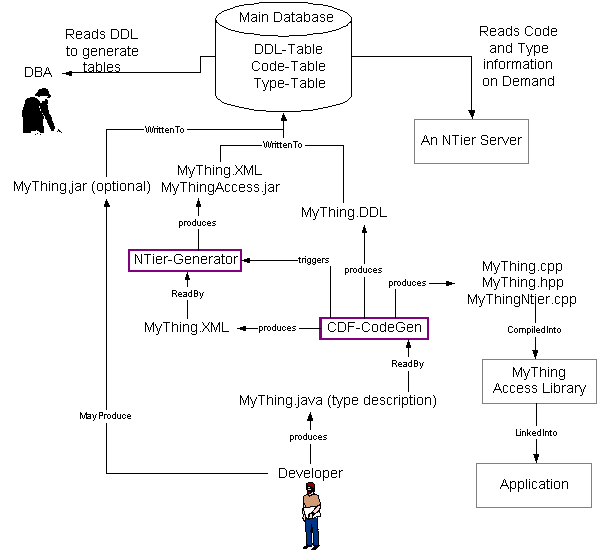
\includegraphics[width=\textwidth]{adding_defs.png}
\caption{Architecture of the \frontier system.
\label{fig:development}}
\end{figure}

The \ref{fig:development} figure shows the flow of information when
a developer adds a new type definition into the system. Developers
attach a release to a specific ntier/database instance.  If the
developer is creating and trying out new definitions, he may be
attached to the development database and ntier instance.  If he
is doing work out of a production release, that release may be
attached to the production database and ntier instance.

Developers are expected to create table/object definitions as they
do today.  In the case of CDF, this mean java-DDL and the CDF code
generation system.  The code generator will need to produce a 
type definition that the ntier system expects in addition to the 
RDBMS-DDL that it already generates.  The build system will need to
run a utility contained in the ntier release that performs the upload
of this ntier type definition into the database.

Developers will have the option of choosing the generic ntier access
generation or to create a custom access library.  For simple data tables
(as in the calibration tables at CDF now), a one-to-one mapping between
object and table may be adequate.  In this case, the developer can choose
to have the ntier access library generated automatically.  If the
new object complicated, such as a view across several tables, then the
developer can supply a custom access library that will map the set of
tables to the desired type.

Here is a summary of some of the important properties of this system:
\begin{enumerate}
\item it allows for more than one instance of the ntier system, each
of which is attached to a set of databases
\item all type definitions and table definitions go into the database
\item DBAs or other priviledged individuals pull DDL out of the database
to generate new tables.
\item The ntier servers retrieve new definitions and code from the database
when they receive requests for types that they know nothing about
\item developers can supply custom access code or choose to have 
the simple generic generated for them.
\end{enumerate}








